\documentclass[12pt,a4paper]{article}
\usepackage[utf8]{inputenc}
\usepackage[L7x]{fontenc}
\usepackage[lithuanian]{babel}
\renewcommand{\ttdefault}{lmtt}
\usepackage{url}
\usepackage{indentfirst}
\urlstyle{restrictedbreak}
\usepackage{parskip}
\setlength{\parindent}{15pt}
\usepackage{graphicx}
\usepackage{relsize}
\usepackage{natbib}
\usepackage{amsmath}
\usepackage{setspace}
\usepackage{amsfonts}
\usepackage{amssymb}
\usepackage{verbatim}
\usepackage[unicode]{hyperref}
\newcommand*{\superscript}[1]{\ensuremath{^\textrm{{\scriptsize #1}}}}
\newcommand*{\subscript}[1]{\ensuremath{_\textrm{{\scriptsize #1}}}}
\newcommand*{\tinysuperscript}[1]{\ensuremath{^\textrm{{\tiny #1}}}}
\newcommand*{\tinysubscript}[1]{\ensuremath{_\textrm{{\tiny #1}}}}
\pagestyle{plain}

\oddsidemargin=0cm
%\topmargin=1cm
\headsep=0pt
\headheight=0pt
\textwidth 6.5in
\textheight 9.00in



%\textheight=640pt
%\footskip=40pt
\newcommand{\mik}{MiK\TeX}
\linespread{1,5}

\newcommand{\eps}{\varepsilon}
\newcommand{\E}{\mathbf{E}}
\newcommand{\PP}{\mathbf{P}}
\title{Particle Swarm Optimization}
\author{Povilas Asijavičius }
\date{Sausis 2015 m.}

\begin{document}

\maketitle

\section{Teorinė dalis}


Paprastai tariant, galima teigti, kad Particle swarm optimization (PSO) algoritmą apibūdina turima populiacija (swarm, būrys) ir galimi sprendiniai (particles, būrio dalelės). Šios dalelės juda po visą nagrinėjamą sritį. Jų judėjimo kryptį nusako kelios nesudėtingos formulės. Dalelių judėjimą lemia jų pačių bei viso būrio rastų optimalių taškų pozicijos. Radus geresnius optimalius taškus visas būrys atsižvelgia į šiuos naujus rezultatus. Procesas tęsiasi tol, kol randamas optimalus taškas arba kol įvykdomas maksimalus iteracijų skaičius.

Kalbant formaliau, galima apibrėžti išlaidų (cost) funkciją $ f: \mathbb{R}^n \rightarrow \mathbb{R}$, kurią sieksime minimizuoti. Ši funkcija kiekvienam vektoriui prisiskirią realią reikšmę. Jos išvestinė nėra žinoma. Priešingu atveju, minimumą būtų galima rasti analiziškai. Taigi tikslas yra rasti tokį sprendinį $x$, kad $f(x) \leq f(y)$, kiekvienam $y$ iš nagrinėjamos erdvės. Norint rasti funkcijos maksimumą, reikėtų minimizuoti funkciją $-f$.

Tarkime, kad S yra dalelių būryje skaičius. Kiekviena iš šių dalelių ($i$-toji) turi dabartinę savo poziciją erdvėje $x_i \in \mathbb{R}^n$ bei greitį $v_i \in \mathbb{R}^n$. Taip pat tariame, kad geriausia žinoma $i$-tosios dalelės pozicija yra $p_i$., o $g_i$ geriausia žinoma visos būrio pozicija. Tada PSO algoritmą galima užrašyti taip:

\begin{itemize}
\item Kiekvienai dalelei $i$, kur $i = 1,..., S$ turime:

\begin{itemize}
\item Nustatome dalelės pradinę poziciją pagal tolygųjį skirstinį $x_i \sim U([b_{il}, b_{iu}])$, kur $b_{il}, b_{iu}$ yra atitinkamai apatinė ir viršutinė nagrinėjamos srities ribos.
\item Geriausia dalelės pozicija nustatome dabartinę jos poziciją $p_i \leftarrow x_i $.
\item Atsitiktinai nustatome dabartinį dalelės greitį $v_i \sim U([-|b_{iu}-b_{il}|, |b_{iu}-b_{il}|])$
\end{itemize}

\item Kol neįvykdoma nustatyta sąlyga (neįvyksta maksimalus iteracijų skaičius arba nėra rastas optimalus taškas) yra vykdoma:

\begin{itemize}
\item Kiekvienai dalelei $i$, kur $i = 1,..., S$ turime:
\begin{itemize}
\item Generuojame atsitiktinius skaičius $r_p, r_g \sim U([0,1])$.
\item Kiekvienam $d$, kur $d = 1,..., n$:
\begin{itemize}
\item atnaujiname dalelės greičius: $v_{id} = \omega v_{id} + \phi_p r_p (p_{id} - x_{id}) + \phi_g r_g (g_{d} - x_{id}) $ 
\end{itemize}
\item Atnaujiname dalelės poziciją: $x_i \leftarrow x_i + v_i$.
\item Jei $ f(x_i) < f(p_i) $:
\begin{itemize}
\item Atnaujiname dalelės geriausią žinomą poziciją $p_i \leftarrow x_i $
\item Jei $ f(p_i) < f(g) $, tai atnaujinama geriausia viso būrio pozicija $g \leftarrow p_i $
\end{itemize}
\end{itemize}
\end{itemize}
\item Dabar $g$ yra geriausias rastas sprendimas.
\end{itemize}


Parametrai $\omega, \phi_p$ ir $\phi_p$ yra parenkami priklausomai nuo situacijos. 


\section{Praktinė dalis}

Toliau bus bandoma pritaikyti ši algoritmą praktiniuose tyrimuose. Parinksime keletą funkcijų ir jas minimizuosime pasirinkus reikiamus parametrus. Darbui naudosime R programą ir jos paketą $pso$. 
Pagrindinė funkcija, kurią naudosime yra $pso$. Jos naudojimas apsirašo taip:


\begin{verbatim*}
psoptim(par, fn, lower = -1, upper = 1, control = list())
\end{verbatim*}

Trumpai apibūdinkime parametrus:

\begin{itemize}
\item $par$ - vektorius nusakantis kokios dimensijos yra erdvė. galima įrašyti tiesiog vektorių su tuščiais elementais. Visgi, jei nurodytos reikšmės paklius į vėliau nustatytas erdvės ribas, tai būtent ši reikšmė bus pradinė reikšmė.
\item $fn$ - funkcija, kuria minimizuojame, funkcijos rezultatas turi būti skaliaras.
\item $lower$  - apatinė kintamojo riba.
\item $upper$  - apatinė kintamojo riba.
\item $control$  - kiti parametrai (tarp jų: maksimalus iteracijų skaičius, konvergavimo tikslumas ir pan.).

\end{itemize}

Toliau išbandykime šią funkciją visiškai paprastam pavyzdžiui:

\begin{spacing}{1}
\begin{verbatim}
> set.seed(1)
> psoptim(c(NA),function(x) x^2-3,lower=-5,upper=5,control=list(abstol=1e-8))
$par
[1] 0.7285336

$value
[1] -2.469239

$counts
 function iteration  restarts 
       12         1         0 

$convergence
[1] 0

$message
[1] "Converged"

\end{verbatim}                                                    
\end{spacing}

\bigskip

Šiuo atveju buvo bandoma rasti minimumą funkcijos $f(x) = x^2 - 3$. Erdvės ribos buvo nustatytos nuo -5 iki 5. Gavome, kad algoritmas konvergavo bet gavo nepatį tiksliausią rezultatą: minimumo taškas yra 0,73 (vietoj 0 iš tikrųjų), funkcijos minimumo taškas -2,47 (-3). Leidžiant simuliaciją daugiau kartų randami ir geresni rezultatai.

Toliau pereikime prie sudėtingesnių situacijų. Bandysime minimizuoti dviejų kintamųjų funkciją:

\begin{equation}
f(x) = 20 + \sum\limits_{i=1}^{2} ( x_i^2 - 10 \cos (2\pi x_i ))
\end{equation}

Kadangi funkcija yra dviejų kintamųjų, mes negalime taip greit nuspėti tikrojo optimumo taško, tačiau mes galime ją pavaizduoti 3D grafike:

\begin{center}
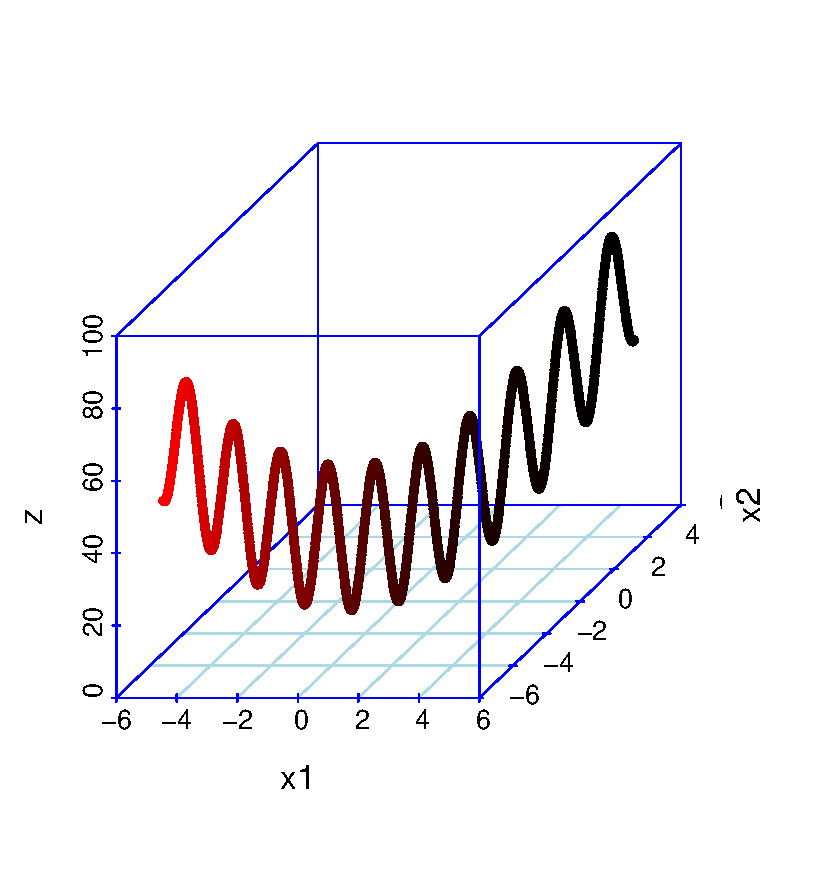
\includegraphics[scale=0.57]{Rplot.pdf}
\end{center}

Grafike gana aiškiai matyti kad minimumas yra maždaug ties reikšme $(0,0)$. Galime pabandyti šį uždavinį išspręst PSO algoritmo pagalba.


\begin{spacing}{1}
\begin{verbatim}
> set.seed(1)
> psoptim(rep(NA,2),function(x) 20+sum(x^2-10*cos(2*pi*x)),
+         lower=-5,upper=5,control=list(abstol=1e-8))
$par
[1]  5.798684e-06 -1.490932e-08

$value
[1] 6.670927e-09

$counts
 function iteration  restarts 
     1404       117         0 

$convergence
[1] 0

$message
[1] "Converged"
\end{verbatim}
\end{spacing}

\bigskip

Matome, kad gavome tikrai gana tikslius rezultatus. $par$ reikšmės yra labai arti nulio, kaip ir pačios funkcijos reikšmė $value$.

Pabandysime minimizuoti dar vieną dviejų kintamųjų funkciją:
\begin{equation}
f(x) = \dfrac{\sum\limits_{i=1}^{2} x_i^2 }{4000} - \sum\limits_{i=1}^{2} \cos \dfrac{x_i}{\sqrt{i}} } +1 
\end{equation}

Vizualizuokime šią funkciją:

\begin{center}
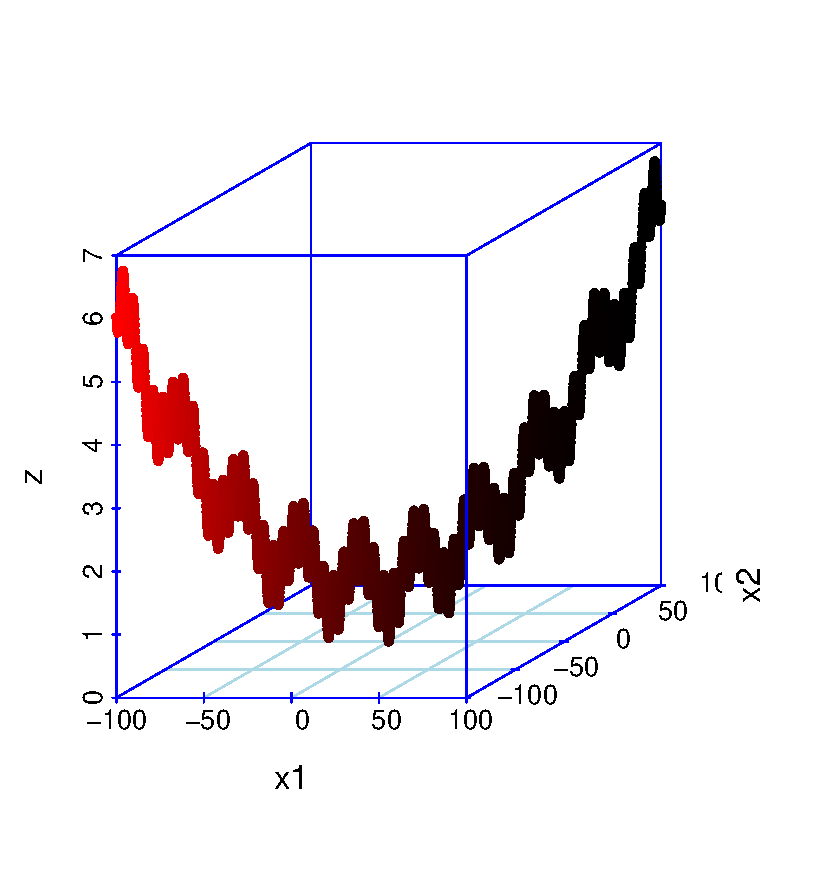
\includegraphics[scale=0.57]{Rplot01.pdf}
\end{center}

Matome, gana panašų vaizdą kaip ir turėjome prieš tai. Pabandykime pritaikyti $pso$:



\begin{spacing}{1}
\begin{verbatim}
> psoptim(rep(NA,2),function(x) sum(x*x)/4000-prod(cos(x/sqrt(1:2)))+1,
+         lower=-100,upper=100,control=list(abstol=1e-2))
$par
[1] -0.04160654 -0.09827913

$value
[1] 0.003279911

$counts
 function iteration  restarts 
     1020        85         0 

$convergence
[1] 0

$message
[1] "Converged"
\end{verbatim}
\end{spacing}

\bigskip

 Matome, kad šiuo atveju rezultatai nėra tokie geri. Įdomu tai, kad paleidus algoritmą daugiau kartų, neretai rezultatai buvo dar blogesni. Tai rodo, kad nepaisant vizualinio panašumo į prieš tai buvusį atvejį, algoritmas šią funkciją minimizuoja kur kas sunkiau .
 






\end{document}



